\section{Nutzerstudie}

\noindent\makebox[\textwidth]{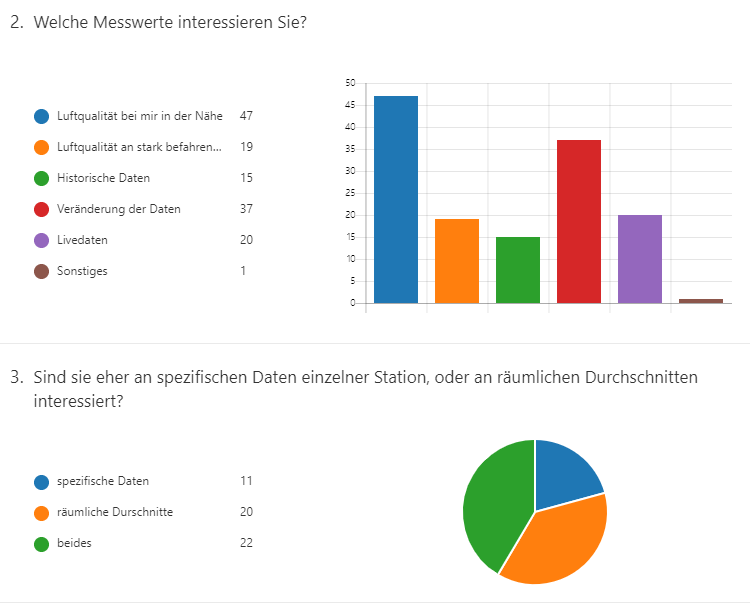
\includegraphics[width=\textwidth]{Umfrage/2,3.png}}
Da 80\% der Befragten sich für die räumlichen Durschnitte interessieren, 
haben wir uns fur die Kartenansicht als Einstiegspunkt für die \gls{Webanwendung} entschieden. 
Dies deckt sich auch mit der größten Interesse nach Luftqualität in der Umgebung von der vorherigen Frage.
\\
\noindent\makebox[\textwidth]{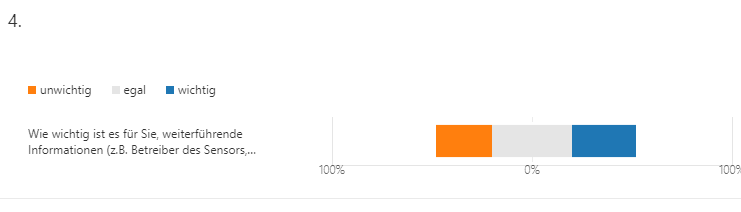
\includegraphics[width=\textwidth]{Umfrage/4.png}} 

\noindent\makebox[\textwidth]{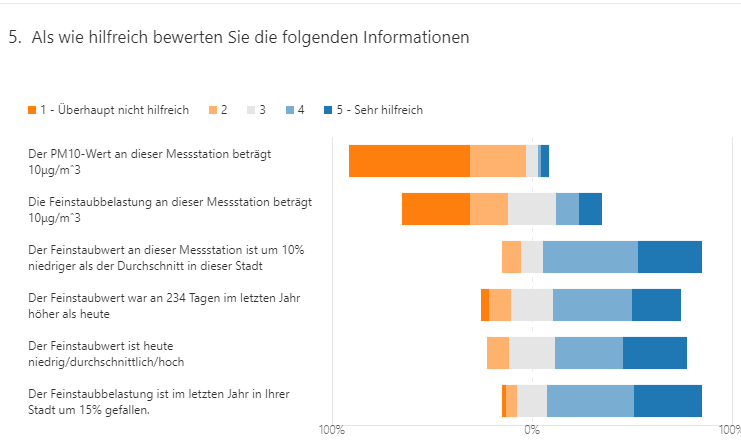
\includegraphics[width=\textwidth]{Umfrage/5.png}}
Hierraus wird ersichtlich das die Befragten eine abstraktere Darstellung der Messwerte hilfreicher finden.
\\
\noindent\makebox[\textwidth]{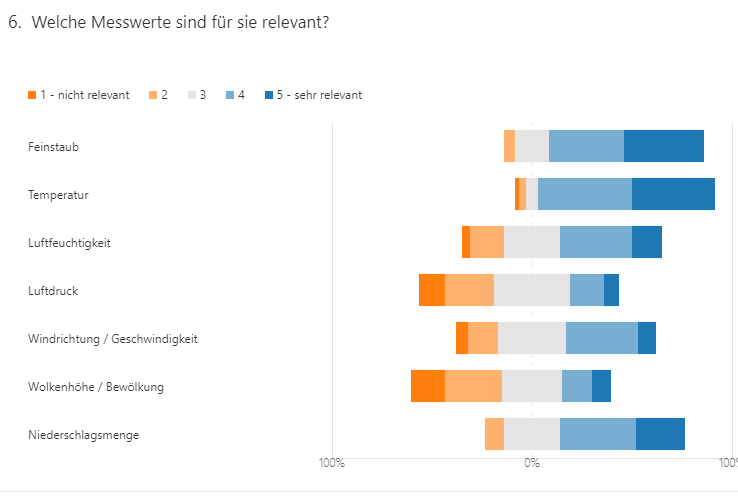
\includegraphics[width=\textwidth]{Umfrage/6.png}}
Die Messwerte mit absteigender Relevanz für die Befragten: 
\\Temperatur, Feinstaub, Niederschlagsmenge, Luftfeuchtigkeit, Wind, Luftdruck und Wolken.
\\ 
\noindent\makebox[\textwidth]{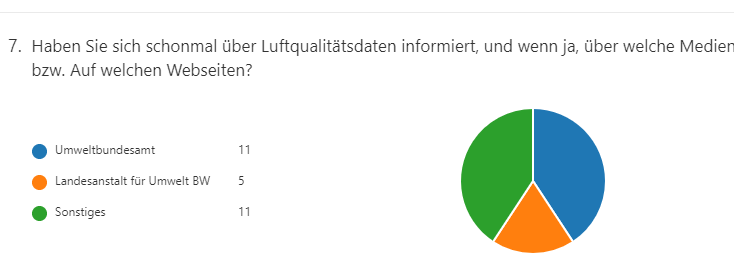
\includegraphics[width=\textwidth]{Umfrage/7.png}}
Sonstige: Nein (6), luftdaten.info (1), Zeitung (1), TV (1), Presse (1), Wetter App (1).
\\
\noindent\makebox[\textwidth]{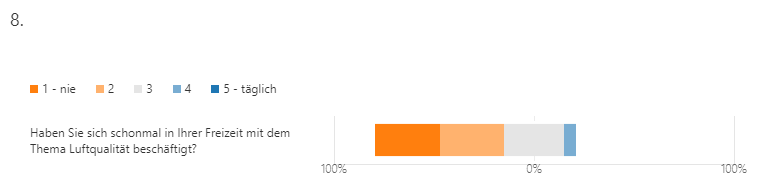
\includegraphics[width=\textwidth]{Umfrage/8.png}}
Die Befragten beschäftigen sich eher selten bis gar nicht mit dem Thema der Luftqualität.
\\
\noindent\makebox[\textwidth]{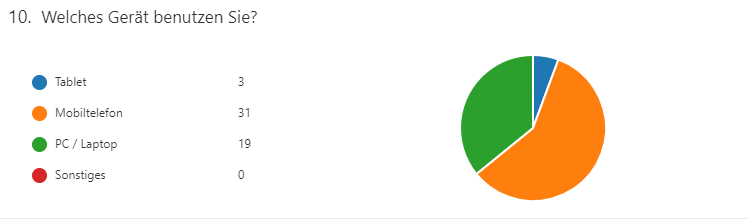
\includegraphics[width=\textwidth]{Umfrage/10.png}}
Die Mehrheit (58\%) der Befragten haben ein Mobiltelefon benutzt. 
Jedoch ist dabei anzumerken, das die Art der Verbreitung der Umfrage eine wesentlichen Einfluss auf das Ergebnis dieser Frage hat. 
Wenn man die Umfrage per WhatsApp auf seinem Smartphone erhält, beantwortet man diese höchstwahrscheinlich auch auf selbigen Gerät.
\\
\noindent\makebox[\textwidth]{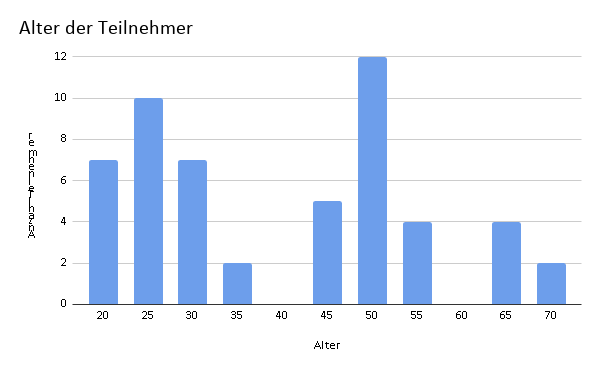
\includegraphics[width=\textwidth]{Umfrage/Alter.png}}
Das Durschnittsalter der Befragten betrug 38 Jahre. Das Alter lag in dem Intervall [18,70]. 
Es haben 53 Menschen an der Umfrage teilgenommen. 